\section{JavaScript Semantics Specialization with Syntactic Views}\label{sec:formal}

We first define $\ires$ as a specification language to describe JavaScript
semantics.  Then, we introduce a general formalization of function
specialization in $\ires$. Finally, we define a constant propagation
specialization as its an instance to reduce JavaScript semantics using given
syntactic views. We also prove its semantics preservation.

\subsection{$\ires$: Intermediate Representations for ECMAScript}

We first introduce $\ires$, an \textbf{I}ntermediate \textbf{R}epresentations
for \textbf{E}CMA\textbf{S}cript, as a specification language for JavaScript to
describe JavaScript semantics. We define its abstract syntax, states, and
concrete semantics in the remainder of this section.

\subsubsection{Abstract Syntax}

\[
  \begin{array}{lr@{~}c@{~}c@{~}c@{~}l}
    \text{Functions} & \funcset &\ni& \func &::=&
    \kwdef \; \varx \; \kwrl \varx^* \kwrr \; \lab\\

    \text{Variables} & \varset &\ni& \varx\\

    \text{Labels} & \labset &\ni& \lab\\

    \text{Instructions} & \instset &\ni& \inst &::=&
    \refer = \expr \mid
    \varx = \expr \kwrl \expr^* \kwrr \mid
    \kwif \; \expr \; \lab \; \lab \mid
    \kwret \; \expr\\

    \text{Expressions} & \exprset &\ni& \expr &::=&
    \pval \mid
    \op \kwrl \expr^* \kwrr \mid
    \kwcl \kwcr \mid
    \refer\\

    \text{References} & \referset &\ni& \refer &::=&
    \varx \mid \expr \kwsl \expr \kwsr\\
  \end{array}
\]

An $\ires$ program $\prog = (\istset, \getinst, \getnext)$ consists of initial
states and two mappings; $\getinst: \labset \rightarrow \instset$ maps labels to
their instructions, and $\getnext: \labset \rightarrow \labset$ maps labels to
their next labels, where a label $\lab \in \labset$ denotes a program point.  A
function $\func \in \funcset$ is defined with its name, parameters, and body
label.  For presentation brevity, we assume that no global variables exist in
this paper.  An instruction $\inst \in \instset$ is an assignment $\refer =
\expr$, a function call $x = \expr \kwrl \expr^* \kwrr$, a branch $\kwif \;
\expr \; \lab \; \lab$, or a return instruction $\kwret \; \expr$.  An
invocation of an abstract algorithm in ECMAScript is compiled to a function call
instruction with a new temporary variable.  We represent loops using branch
instructions with cyclic pointing of labels in $\getnext$.  An expression is a
primitive value $\pval$, an operation $\op \kwrl \expr^* \kwrr$, an object
allocation $\kwcl \kwcr$, or a reference $\refer$.  A reference is a variable
$x$ or an object field $\expr \kwsl \expr \kwsr$.  We write $\expr.\varf$ to
briefly represent $\expr \kwsl \code{"f"} \kwsr$.


\subsubsection{States}

\[
  \begin{array}{lr@{~}c@{~}l@{~}c@{~}l}
    \text{States} & \st &\in& \stset &=&
    \labset \times \ctxtset^* \times \heapset \times \envset\\

    \text{Calling Contexts} & \ctxt &\in& \ctxtset &=&
    \labset \times \envset \times \varset\\

    \text{Heaps} & \heap &\in& \heapset &=&
    \addrset \finmap \objset\\

    \text{Objects} & \obj &\in& \objset &=&
    \strset \finmap \valset\\

    \text{Environments} & \env &\in& \envset &=&
    \varset \finmap \valset\\

    \text{Values} & \val &\in& \valset &=&
    \pvalset \uplus \addrset \uplus \treeset \uplus \funcset\\

    \text{Primive Values} & \pval &\in& \pvalset &=&
    \boolset \uplus \strset \uplus \cdots\\

    \text{JavaScript ASTs} & \tree &\in& \treeset &::=& \\
  \end{array}
\]

States $\stset$ consist of labels $\labset$, calling context stacks
$\ctxtset^*$, heaps $\heapset$, and environments $\envset$.  A calling context
$\ctxt \in \ctxtset$ consists of a label denoting the return point, a caller's
environment, and a return variable.  A heap $\heap \in \heapset$ is a finite
mapping from addresses to objects, and an object $\obj \in \objset$ is a finite
mappings from strings to values.  Each object allocation $\kwcl \kwcr$ creates a
unique address $\addr \in \addrset$ different from existing addresses.  An
environment $\env \in \envset$ is a finite mapping from variables to values. A
value $\val \in \valset$ is a primitive value $\pval \in \pvalset$ (e.g., a
boolean value $\bool \in \boolset$ or a string value $\str \in \strset$), an
address $\addr \in \addrset$, a JavaScript AST $\tree \in \treeset$, or a
function $f \in \funcset$.

Since $\ires$ is a specification language for JavaScript, it treats JavaScript
ASTs $\treeset$ as its values. For presentation brevity, we represent a JavaScript
AST as follows:
\[
  \tree ::= \str \mid \ty_k \langle \tree^* \rangle
\]
A string $\str$ denotes a leaf node with a terminal symbol, and $\ty_k \langle
\tree^* \rangle$ denotes a non-leaf node for $k$-th alternative in the syntactic
production of nonterminal symbol $\ty$ with its subtrees $\tree^*$.  The notation
$\ty_k.\eval$ denotes an $\ires$ function for the evaluation of $k$-th
alternative in $\ty$, and it takes the AST itself and its nonterminal subtrees
as arguments. For each integer $k$, the notation $\tree[k]$ denotes $k$-th
subtree of $\tree$.  For example, Figure~\ref{fig:coalesce-prod} shows a
syntactic production for coalesce expressions.  Consider the following coalesce
expression:
\begin{lstlisting}[style=JS]
                    42 ?? true
\end{lstlisting}
Then, the following AST is produced as its parsing result:
\begin{figure}[H]
  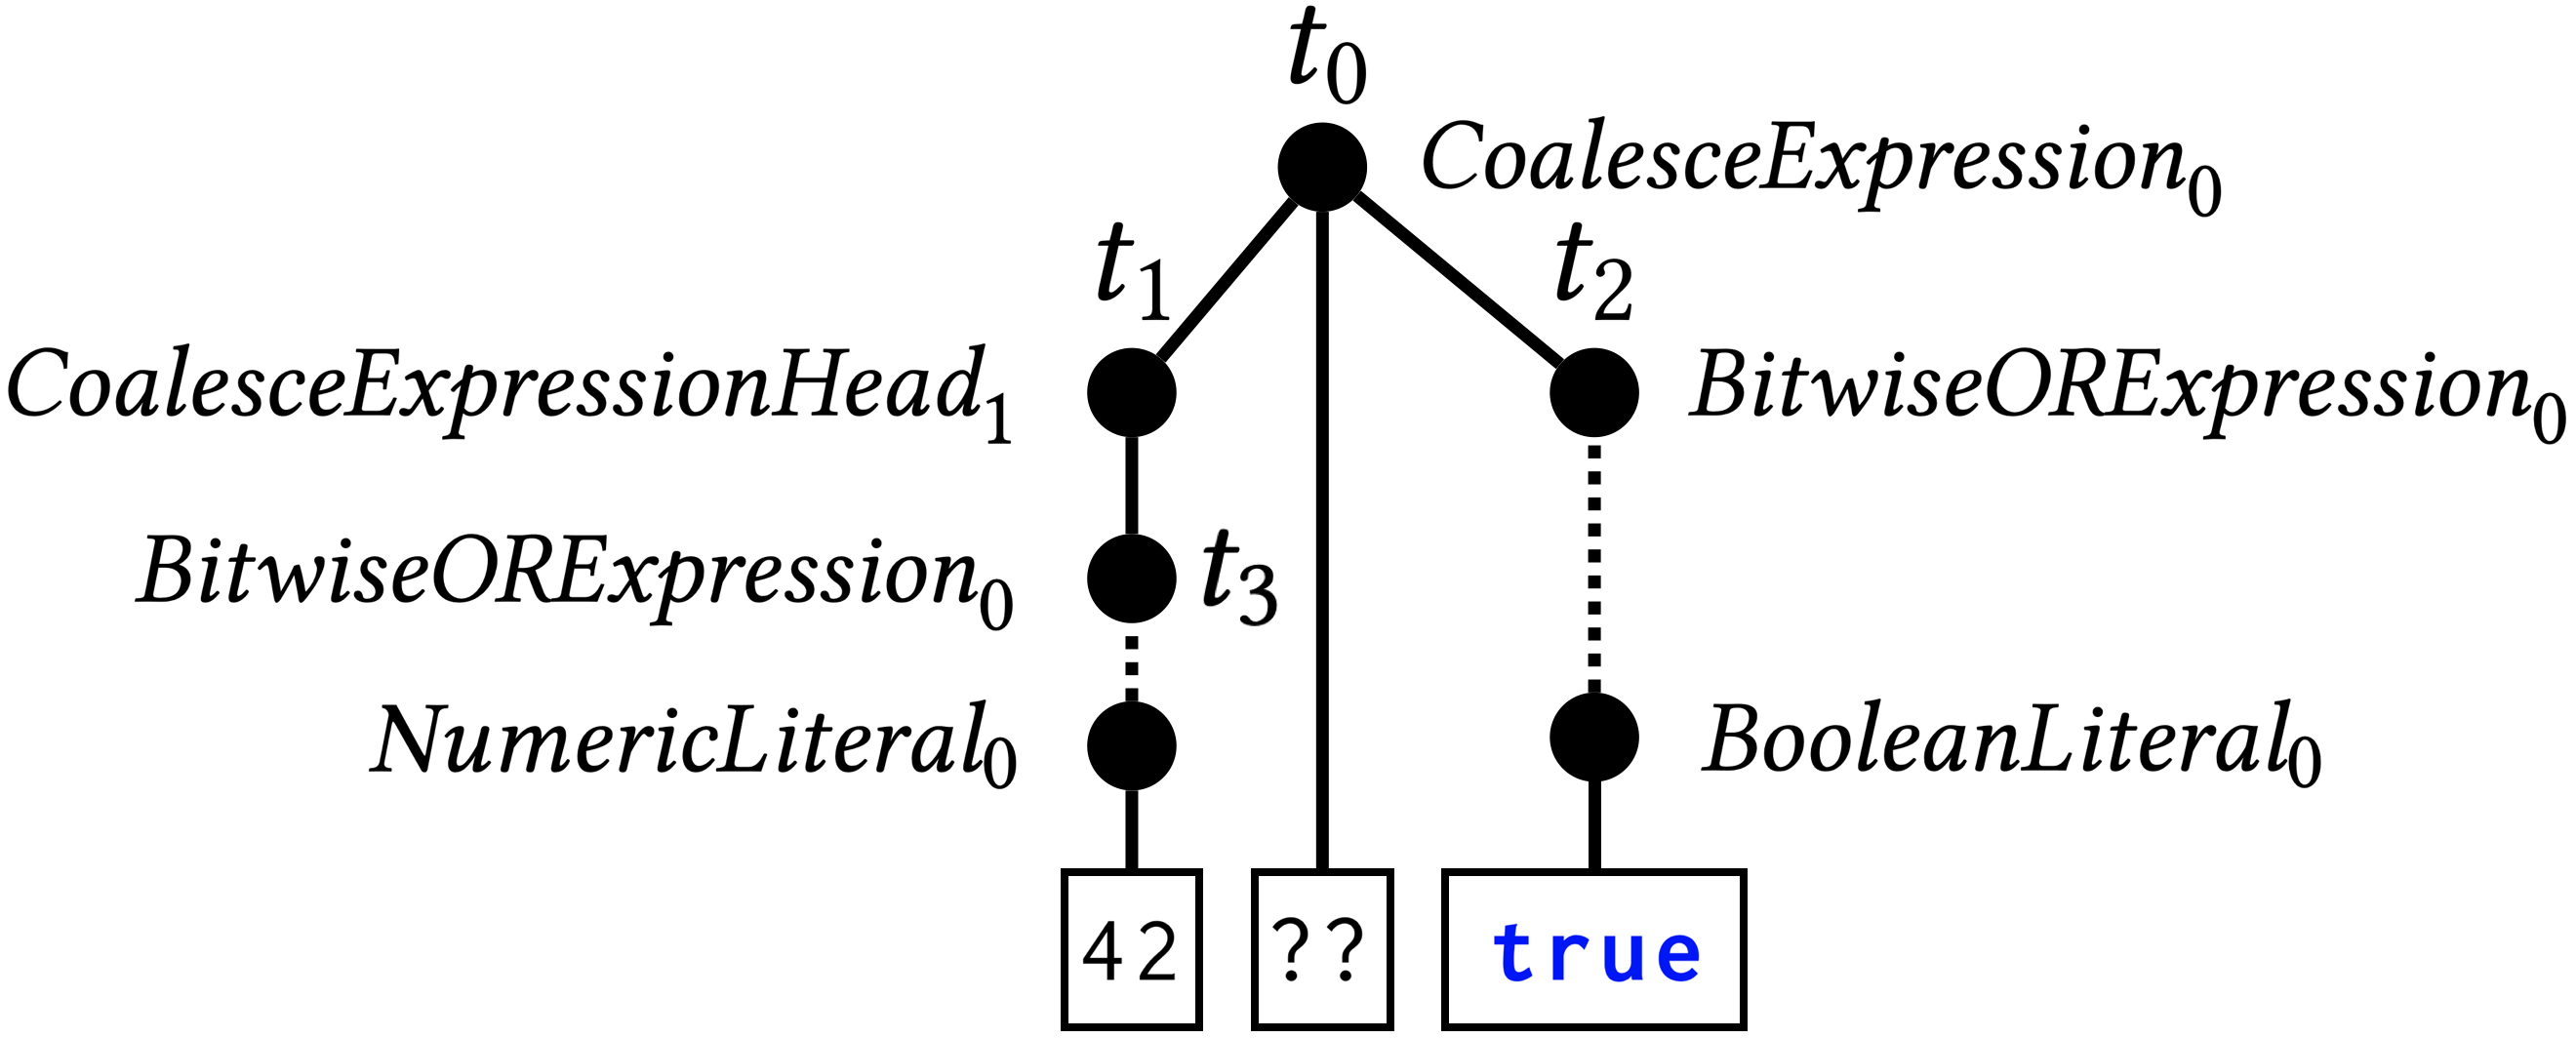
\includegraphics[width=.8\columnwidth]{img/ast-example.png}
\end{figure}
\noindent Moreover, its evaluation function $\nterm{CoalesceExpression}_0.\eval$
takes three subtrees as arguments annotated by $\tree_0$, $\tree_1$, and
$\tree_2$ in the AST.


\begin{figure}
  \centering
  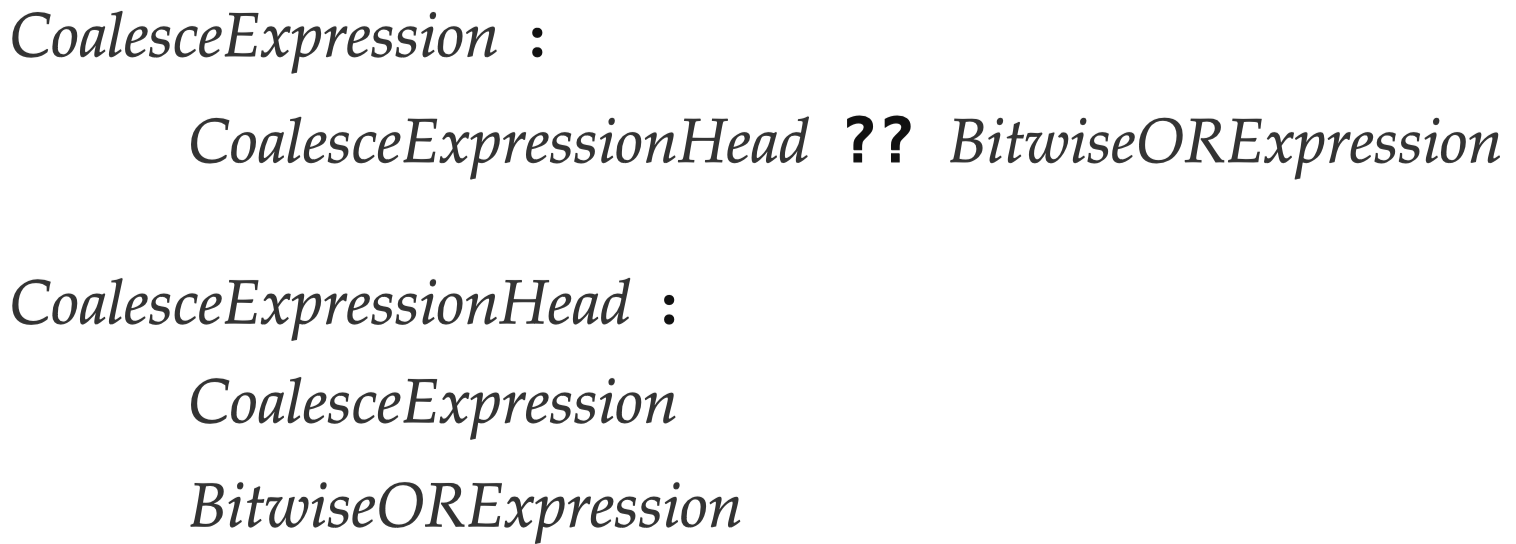
\includegraphics[width=.8\columnwidth]{img/coalesce-prod.png}
  \caption{A JavaScript syntactic production for coalesce expressions}
  \label{fig:coalesce-prod}
\end{figure}




\subsubsection{Concrete Semantics}

The concrete semantics $\sem{\prog}$ of an $\ires$ program $\prog = (\istset,
\getinst, \getnext)$ is defined as follows:
\[
  \sem{\prog} = \{ \st \in \stset \mid \ist \in \istset \wedge \ist \trans^* \st \}
\]
where $\trans^*$ denotes one or more repetition of $\trans$, and $\st \trans
\st'$ if and only if $\st = (\lab, \_, \_, \_)$ and $\sem{\getinst(\lab)}(\st) =
\st'$. Now, we define the denotational semantics of instructions $\sem{\inst}:
\stset \rightarrow \stset$ and expressions $\sem{\expr}: \stset \rightarrow
\stset \times \valset$.

\todo function semantics

\paragraph{Instructions}
\[
  \framebox{$\sem{\inst}: \stset \rightarrow \stset$}
\]
\begin{itemize}
  \item \underline{Variable Assignments}:
    \[
      \sem{\varx = \expr}(\st) =
      (\getnext(\lab), \ctxts, \heap, \env[\varx \mapsto \val])
    \]
    where
    \[
      \sem{\expr}(\st) = ((\lab, \ctxts, \heap, \env), \val)
    \]

  \item \underline{Field Assignments}:
    \[
      \sem{\expr_0 \kwsl \expr_1 \kwsr = \expr_2}(\st) =
      (\getnext(\lab), \ctxts, \heap[\addr \mapsto \obj'], \env)
    \]
    where
    \[
      \begin{array}{l@{~}c@{~}ll}
        \sem{\expr_0}(\st) &=& (\st', \addr) &\wedge\\
        \sem{\expr_1}(\st') &=& (\st'', \str) &\wedge\\
        \sem{\expr_2}(\st'') &=& ((\lab, \ctxts, \heap, \env), \val) &\wedge\\
        \obj &=& \heap(\addr) &\wedge\\
        \obj' &=& \obj[\str \mapsto \val]\\
      \end{array}
    \]

  \item \underline{Function Calls}:
    \[
      \sem{\varx = \expr \kwrl \expr_1 \cdots \expr_n \kwrr}(\st) =
      (\lab_\varf, \ctxt :: \ctxts, \heap, \env')
    \]
    where
    \[
      \begin{array}{l@{~}c@{~}ll}
        \sem{\expr}(\st) &=& (\st_0, \kwdef \; \varf \; \kwrl \varp_1, \cdots,
        \varp_n \kwrr \; \lab_\varf) &\wedge\\
        \sem{\expr_k}(\st_{k-1}) &=& (\st_k, \val_k) \; \forall 1 \leq k \leq n
        &\wedge\\
        \st_n &=& (\lab, \ctxts, \heap, \env) &\wedge\\
        \env' &=& [\varp_1 \mapsto \val_1, \cdots, \varp_n \mapsto \val_n]
        &\wedge\\
        \ctxt &=& (\getnext(\lab), \env, \varx)\\
      \end{array}
    \]

  \item \underline{Branches}:
    \[
      \sem{\kwif \; \expr \; \lab_\vart \; \lab_\varf}(\st) =
      \left\{
        \begin{array}{ll}
          (\lab_\vart, \ctxts, \heap, \env) & \text{if} \; \val = \true\\
          (\lab_\varf, \ctxts, \heap, \env) & \text{if} \; \val = \false\\
        \end{array}
      \right.
    \]
    where
    \[
      \sem{\expr}(\st) = ((\lab, \ctxts, \heap, \env), \val)
    \]

  \item \underline{Returns}:
    \[
      \sem{\kwret \; \expr}(\st) = (\lab, \ctxts, \heap, \env[\varx \mapsto
      \val])
    \]
    where
    \[
      \sem{\expr}(\st) = ((\_, (\lab, \env, \varx) :: \ctxts, \heap, \_), \val)
    \]
\end{itemize}

\paragraph{Expressions}
\[
  \framebox{$\sem{\expr}: \stset \rightarrow \stset \times \valset$}
\]
\begin{itemize}
  \item \underline{Primive Values}:
    \[
      \sem{\pval}(\st) =
      (\st, \pval)
    \]

  \item \underline{Operations}:
    \[
      \sem{\op \kwrl \expr_1, \cdots, \expr_n \kwrr}(\st) =
      (\st_n, \op(\val_1, \cdots, \val_n))
    \]
    where
    \[
      \st_0 = \st \wedge
      \forall 1 \leq k \leq n. \; \sem{\expr_k}(\st_{k-1}) = (\st_k, \val_k)
    \]

  \item \underline{Object Allocations}:
    \[
      \sem{\kwcl \kwcr}(\st) =
      ((\lab, \ctxts, \heap[\addr \mapsto \varnothing], \env), \addr)
    \]
    where
    \[
      \st = (\lab, \ctxts, \heap, \env) \wedge
      \addr \not\in \text{Domain}(\heap)
    \]

  \item \underline{Variable Lookups}:
    \[
      \sem{\varx}(\st) =
      (\st, \env(\varx))
    \]
    where
    \[
      \st = (\_, \_, \_, \env)
    \]

  \item \underline{Field Lookups}:
    \[
      \sem{\expr_0 \kwsl \expr_1 \kwsr}(\st) =
      (\st'', \val')
    \]
    where
    \[
      \begin{array}{l@{~}c@{~}ll}
        \sem{\expr_0}(\st) &=& (\st', \addr) &\wedge\\
        \sem{\expr_1}(\st') &=& (\st'', \str) &\wedge\\
        \st'' &=& (\_, \_, \heap, \_) &\wedge\\
        \obj &=& \heap(\addr) &\wedge\\
        \val' &=& \obj(\str)\\
      \end{array}
    \]
\end{itemize}





\subsection{Function Specialization}

A \textit{function specialization} is defined with the following three
components:
\begin{itemize}
  \item Restriction $\restrictset$
  \item Concretization $\gamma: \restrictset \rightarrow \powerset{\stset
    \times \valset^*}$
  \item Transformation $\transform: \restrictset \rightarrow \funcset
    \rightarrow \funcset$.
\end{itemize}
We can restrict possible input states and arguments of functions by defining a
set of restrictions $\restrictset$ with their concretization $\gamma:
\restrictset \rightarrow \powerset{\stset \times \valset^*}$. A transformation
$\transform: \restrictset \rightarrow \funcset \rightarrow \funcset$ is
parameteric with such restrictions and transforms a function to another function
by preserving semantics under a given restriction.


\subsubsection{Constant Propagation Specialization}
We define a \textit{constant propagation specialization} with the following
three components:

\begin{itemize}
  \item Restriction $\cprestrictset = \avalset^*$
  \item Concretization $\cpgamma: \avalset^* \rightarrow \powerset{\stset
    \times \valset^*}$ s.t.
    \[
      \cpgamma(\aval_1, \cdots, \aval_n) =
      \stset \times (\valgamma(\aval_1) \times \cdots \times \valgamma(\aval_n))
    \]
  \item Transformation $\cptransform: \avalset^* \rightarrow \funcset
    \rightarrow \funcset$
\end{itemize}
The constant propagation specialization restricts specific arguments with
concrete values with a restriction defined with a sequence of static or dynamic
values $\valset \uplus \{ \top \}$, but it does not restrict input states.
While a dynamic value $\top$ denotes no restriction, it restricts a specific
argument with the static value $\val \in \valset$. To specialize functions under
a given restriction $(\aval_1, \cdots, \aval_n) \in \avalset^*$, we
define a transformation $\cptransform: \avalset^* \rightarrow \funcset
\rightarrow \funcset$. To propagate constants, \todo What is a constant?
a constant is a value which is statically fixed under a given restriction.

\[
  \begin{array}{lr@{~}c@{~}l@{~}c@{~}l}
    \text{Abstract Environments} & \aenv &\in& \aenvset &=&
    \varset \rightarrow \avalset\\
    \text{Abstract Values} & \aval &\in& \avalset &=&
    (\valset \times \exprset) \uplus \{ \bot, \top \}\\
  \end{array}
\]

\todo $\envgamma, \valgamma, \join, \meet, \order$

\paragraph{Expressions}
\[
  \framebox{$\asem{\expr}: \aenvset \rightarrow \avalset$}
\]
\begin{itemize}
  \item \underline{Primive Values}:
    \[
      \asem{\pval}(\aenv) = (\pval, \pval)
    \]
  \item \underline{Operations}:
    \[
      \asem{\op \kwrl \expr_1, \cdots, \expr_n \kwrr}(\aenv) =
      (\aval, \expr)
    \]
    where
    \[
      \begin{array}{l@{~}c@{~}ll}
        \asem{\expr_k}(\aenv) &=& \aval_k \; \forall 1 \leq k \leq n
        &\wedge\\
        \aval &=& \left\{
          \begin{array}{ll}
            \bot & \text{if} \; \exists k. \; \aval_k = \bot\\
            \top & \text{if} \; \exists k. \; \aval_k = \top\\
            (\val, \expr') &
            \text{if} \; \forall k. \; \aval_k = (\val_k, \expr'_k)\\
          \end{array}
        \right. &\wedge\\
        \val &=& \op(\val_1, \cdots, \val_n) &\wedge\\
        \expr' &=& \op(\expr'_1, \cdots, \expr'_n)\\
      \end{array}
    \]
  \item \underline{Object Allocations}:
    \[
      \asem{\kwcl \kwcr}(\aenv) = \top
    \]
  \item \underline{Variable Lookups}:
    \[
      \asem{\varx}(\aenv) = \aenv(\varx)
    \]
  \item \underline{Field Lookups}:
    \[
      \asem{\expr_0 \kwsl \expr_1 \kwsr}(\aenv) = \top
    \]
\end{itemize}
\[
  \framebox{$\cptransforme: \exprset \times \aenvset \rightarrow \exprset \times
  \avalset$}
\]
\[
  \cptransforme(\expr, \aenv) = (\expr'', \aval)
\]
where
\[
  \begin{array}{l@{~}c@{~}ll}
    \aval &=& \asem{\expr}(\aenv) &\wedge\\
    \expr'' &=& \left\{
      \begin{array}{ll}
        \pval & \text{if} \; \aval = (\pval, \_)\\
        \expr' & \text{if} \; \aval = (\_, \expr')\\
        \expr & \text{otherwise}\\
      \end{array}
    \right.\\
  \end{array}
\]

\paragraph{Instructions}
\[
  \framebox{$\cptransformi: \instset \times \aenvset \rightarrow \instset \times
  \aenvset$}
\]
\begin{itemize}
  \item \underline{Variable Assignments}:
    \[
      \cptransformi(\varx = \expr, \aenv) =
      (\varx = \expr', \aenv[\varx \mapsto \aval])
    \]
    where
    \[
      (\expr', \aval) = \cptransforme(\expr, \aenv)
    \]

  \item \underline{Field Assignments}:
    \[
      \cptransformi(\expr_0 \kwsl \expr_1 \kwsr = \expr_2, \aenv) =
      (\expr'_0 \kwsl \expr'_1 \kwsr = \expr'_2, \aenv)
    \]
    where
    \[
      \begin{array}{l@{~}c@{~}ll}
        (\expr'_0, \_) = \cptransforme(\expr_0, \aenv) &\wedge\\
        (\expr'_1, \_) = \cptransforme(\expr_1, \aenv) &\wedge\\
        (\expr'_2, \_) = \cptransforme(\expr_2, \aenv)\\
      \end{array}
    \]

  \item \underline{Function Calls}:
    \[
      \cptransformi(\varx = \expr \kwrl \expr_1 \cdots \expr_n \kwrr, \aenv) =
      (\varx = \expr' \kwrl \expr'_1 \cdots \expr'_n \kwrr,
      \aenv[\varx \mapsto \top])
    \]
    where
    \[
      \begin{array}{l@{~}c@{~}ll}
        (\expr', \_) = \cptransforme(\expr, \aenv) &\wedge\\
        (\expr'_k, \_) = \cptransforme(\expr_k, \aenv) \; \forall 1 \leq k \leq
        n\\
      \end{array}
    \]

  \item \underline{Branches}:
    \[
      \cptransformi(\kwif \; \expr \; \lab_\vart \; \lab_\varf, \aenv) =
      (\kwif \; \expr' \; \lab_\vart \; \lab_\varf, \aenv)
    \]
    where
    \[
      (\expr', \_) = \cptransforme(\expr, \aenv)
    \]

  \item \underline{Returns}:
    \[
      \cptransformi(\kwret \; \expr, \aenv) =
      (\kwret \; \expr, \aenv)
    \]
    where
    \[
      (\expr', \_) = \cptransforme(\expr', \aenv)
    \]
\end{itemize}

\paragraph{Functions}
\[
  \framebox{$\cptransform: (\avalset)^* \rightarrow \funcset \rightarrow
  \funcset$}
\]

\todo





% \subsubsection{Redundancy Elimination Transformation}
% 
% \[
%   \begin{array}{lr@{~}c@{~}l}
%     \text{Restrictions} &\{ \top \}\\
%     \text{Concretization} & \gamma(\top) &=& \stset \times \valset^*\\
%   \end{array}
% \]
% 
% The redundancy elimination transformation is defined without any restriction,
% which means its restriction set consists of a single element $\top$
% representing all possible cases.  Therefore, we omit the restriction part in
% this transformation for the brevity.
% 
% \[
%   \framebox{$\transformref: \funcset \rightarrow \funcset$}
% \]
% 
% \todo








\subsection{Proof of Semantics Preservation}

\todo





\subsection{JavaScript Semantics Specialization}

This section explains how to utilize the constant propagation specialization for
the JavaScript semantics specialization with a user-defined syntactic view.  We
first formally define syntactic views and their operations, then we explain how
to decide a restriction of the constant propagation specialization based on a
given syntactic view.

\subsubsection{Syntatic Views}

\todo

\subsubsection{Specialization with Syntatic Views}

\todo
